\chapter{BDTG output variation with \CV and \Ct }\label{sec:bdtvscvct}

The BDTG classifier output was described in Section \label{secc:signal_disc} in the \Ct=-1,\CV=1 scenario; the change of BDTG classifiers output shape when varying the \CV/\Ct\ coupling scenario is shown in Figure~\ref{fig:bdtvscvct} in the $3l$ channel for five different values of \Ct, with \CV\ fixed at $1.0$.
\begin{figure} [!h]
  \centering
  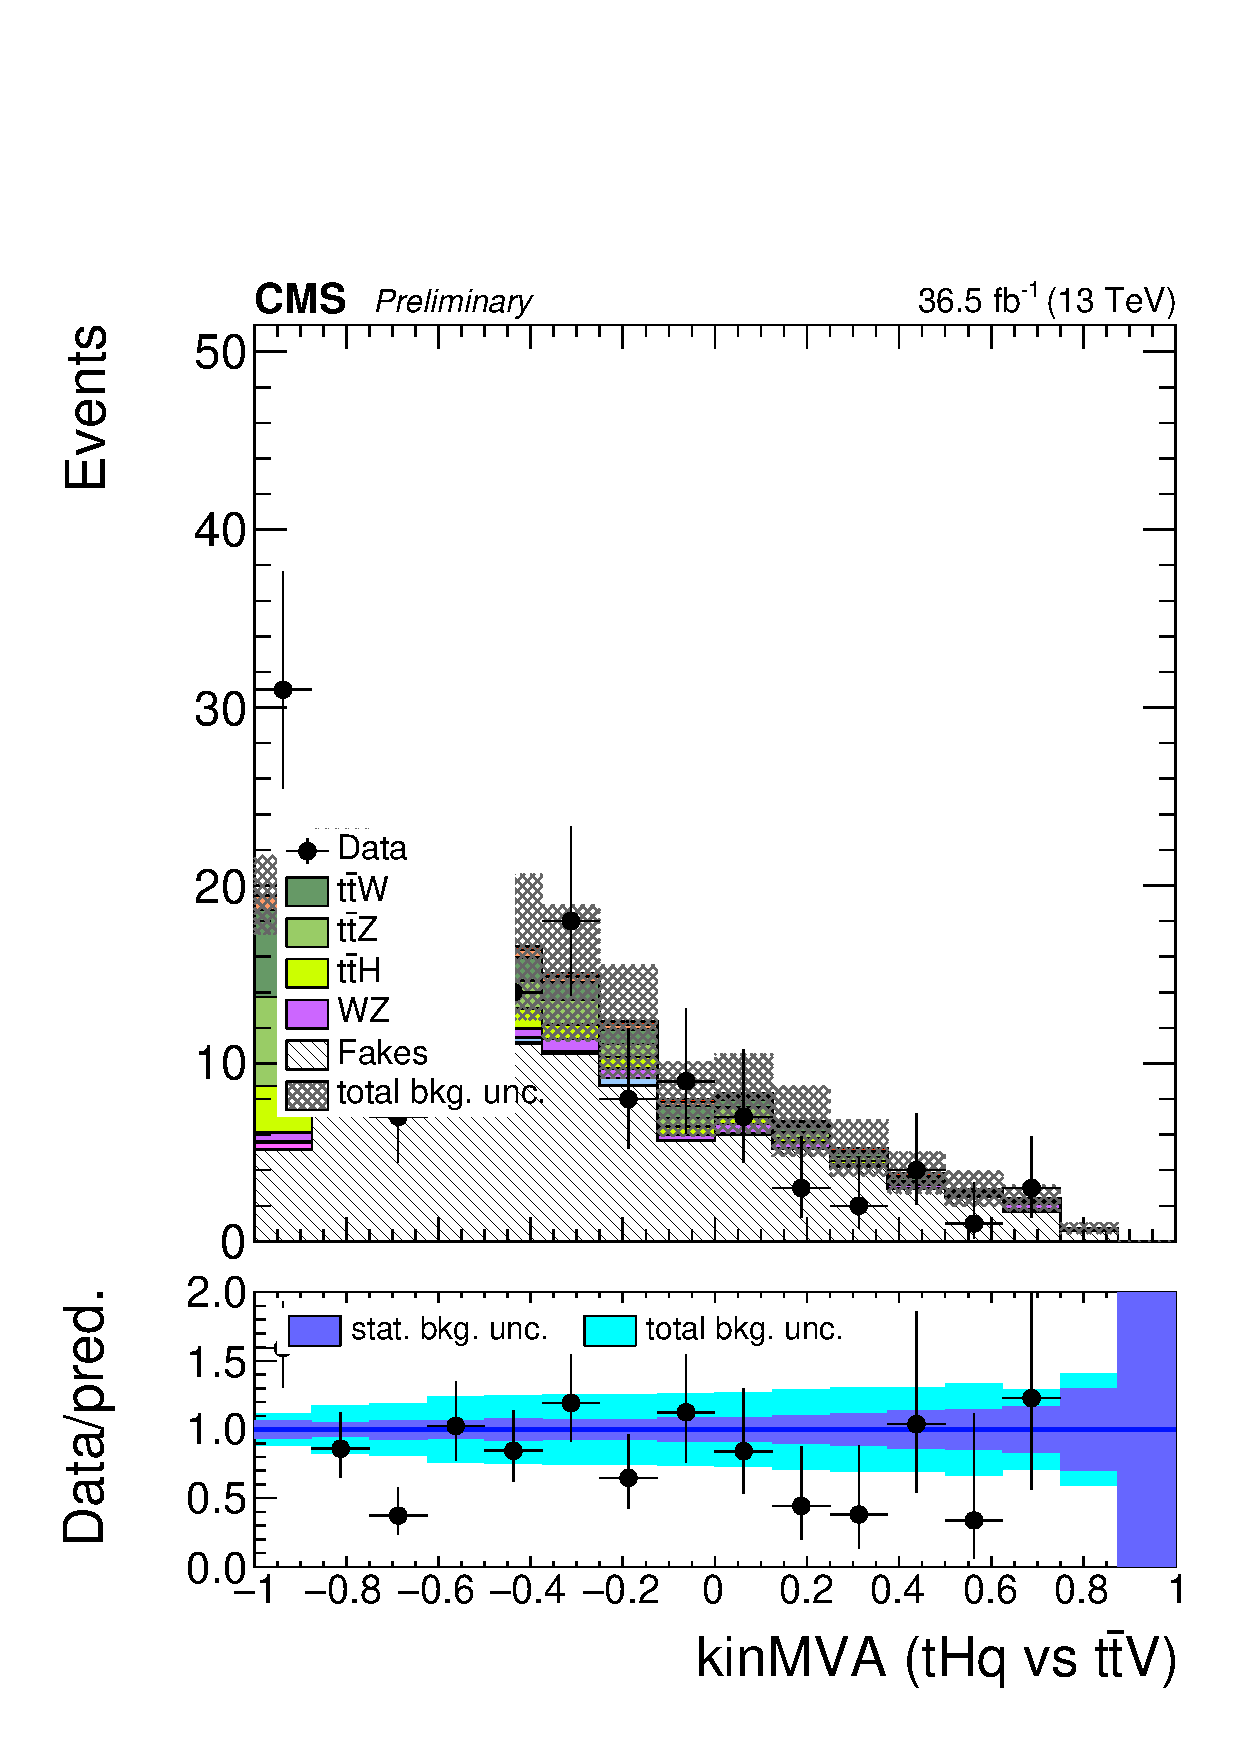
\includegraphics[width=0.45\textwidth]{controlplots/bdtvscvct/thqMVA_ttv_3l.pdf}
  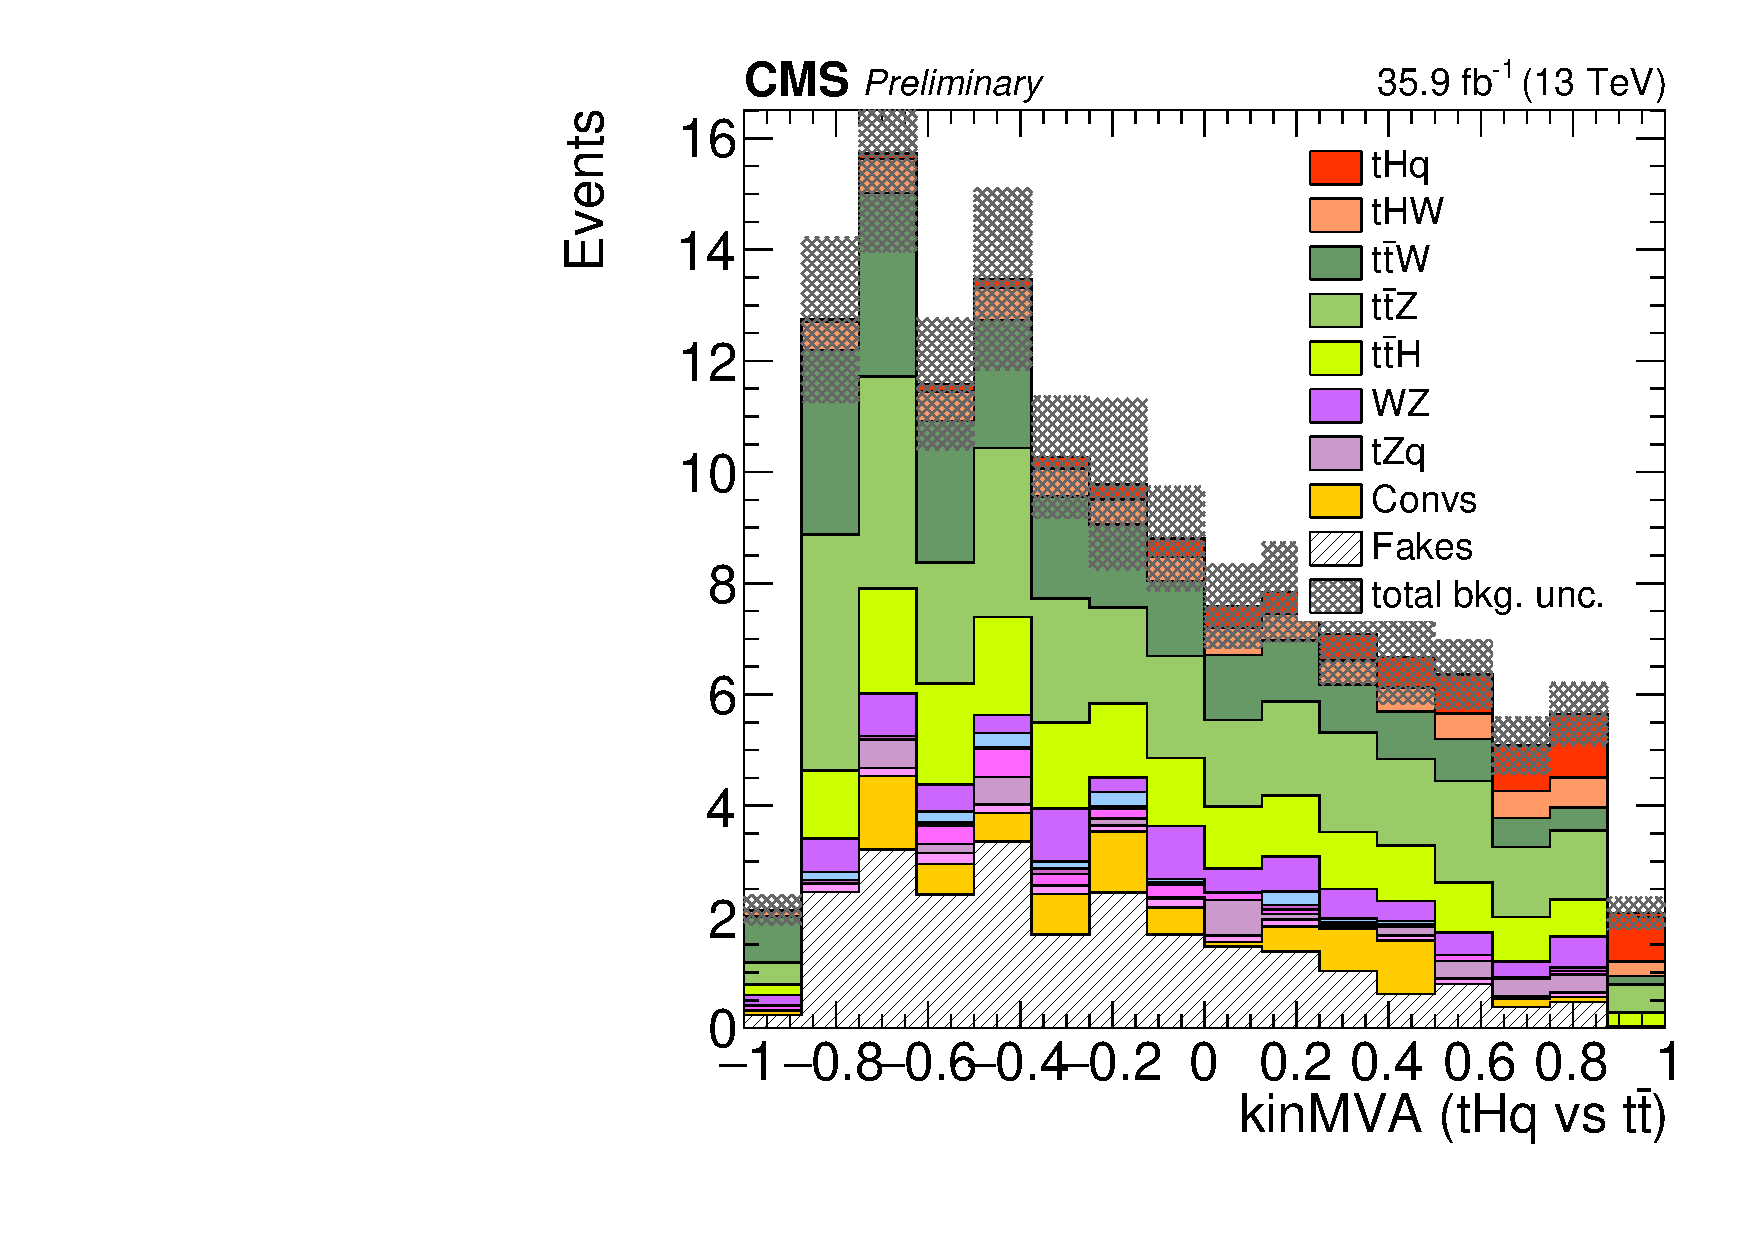
\includegraphics[width=0.45\textwidth]{controlplots/bdtvscvct/thqMVA_tt_3l.pdf} \\
  \caption[BDTG output variation with \CV/\Ct]{Change of the BDTG classifiers output when varying \Ct\ coupling (\CV\ is fixed at $1.0$). Training vs.\ \ttV\ (right) and vs.\ \ttbar\ (left).}
  \label{fig:bdtvscvct}
\end{figure}

Given that the BDT classifier output shape does not change, it is enought to train the BDTG in one of the \Ct/\CV points. It was chosen the SM point.  

